%!TEX root=paper.tex

\section{Retrospective and Prospective Remarks}
\label{sec:conc}

\paragraph{Retrospective} As a promising first step, my proposal explores the feasibility of a holistic system design to improve the power-efficiency of active timing margin processors while maintaining legacy system interfaces and ensuring reliability. 

My proposal argues that to maximize the power efficiency benefits of active timing margin processors, synergy among circuit design, firmware design, as well as application scheduling is needed. It demonstrates three general principles in my research:

\begin{itemize}
  \item \textsc{Measuring Timing Margin Opportunity~~} Solid research starts from rigid measurement of the opportunity that lies beneath a potential problem. Our measurement on state-of-the-art hardware identifies the power reduction opportunity from excess timing margin, as well as the deficiency of existing active timing processors. These measurement and characterization serve as the starting point of our work.
    
  \item \textsc{Identifying Root Causes~~} Before delivering solutions that improve timing margin efficiency, the root cause of the current problem, whether it's excess margin for temperature variation, or scalability issue of existing active timing margin processors, must be found out. The final solution needs to address the root cause properly in order to be effective. The process to identify the root cause is complex, and sometimes involve stripping down multiple factors one by one as what we did in AMS. Yet, it is a necessary step in maintaining reliability while improving processor efficiency.
    
  \item \textsc{Succinct Solution Design Across Stack~~} To management active timing margin, solutions across the stack, ranging from circuit design, to firmware power states, to application scheduling logic, are proposed. Each solution is unique and makes sense in its own implementation form - dealing with $di/dt$ effect in hardware is the only reasonable way, whereas storing power states in firmware is cost effective. In AMS, application scheduling is the most convenient approach without intrusive hardware re-design. In this proposal, we try to make the end solution easy to implement and evaluate.
  
\end{itemize}

\paragraph{Prospective} As my next step towards defense, I plan to extend my  work presented in this proposal to include a ``limit analysis'' of active timing margin solutions. We call this limit analysis \textit{EnergySecure}. The name encompasses the implication of this work - to reduce energy and improve power efficiency, while making sure system is still secure/reliable in its ``edge'' state.

At a high level, \textit{EnergySecure} pushes the ``safety margin'' in active timing margin to the limit to squeeze the last bit of power efficiency benefits from wasted margin. The ``safety margin'' here refers to the timing margin left in active timing margin. In the analogy of car and lane width, active timing margin will dynamically adjust lane width to match the car's orbit, just as how processor adjust voltage and frequency to account for temperature and voltage variation. Yet, even though the lane width is adjusted on-the-fly, there should still be a ``safety space'' between car's silhouette and the lane. This ``safety space'' exists because there is no way we can guarantee the dynamically adjustable lane can always match the car's trace with zero mistake, although now the ``safety space'' is much smaller than that in the original static margin setting. In active timing margin, there is still a small ``timing margin'' left in the system, although the amount of the left ``timing margin'' is much smaller than the original system. The goal of \textit{EnergySecure} is to quantify how much opportunity there is in the timing margin left in active timing margin, and to investigate what we can do to safely squeeze all the timing margin left.

In active timing margin processors, timing margin sensors instructs the operation of the feedback loop that tolerates all sorts of variations. The ``safety margin'' is also configured in the timing margin sensor. In the case of POWER7+, critical path monitors (CPM) implements how much ``safety margin'' is allocated.~\Fig{fig:cpm-internal} illustrates this process.

\begin{figure}[t]
  \centering
  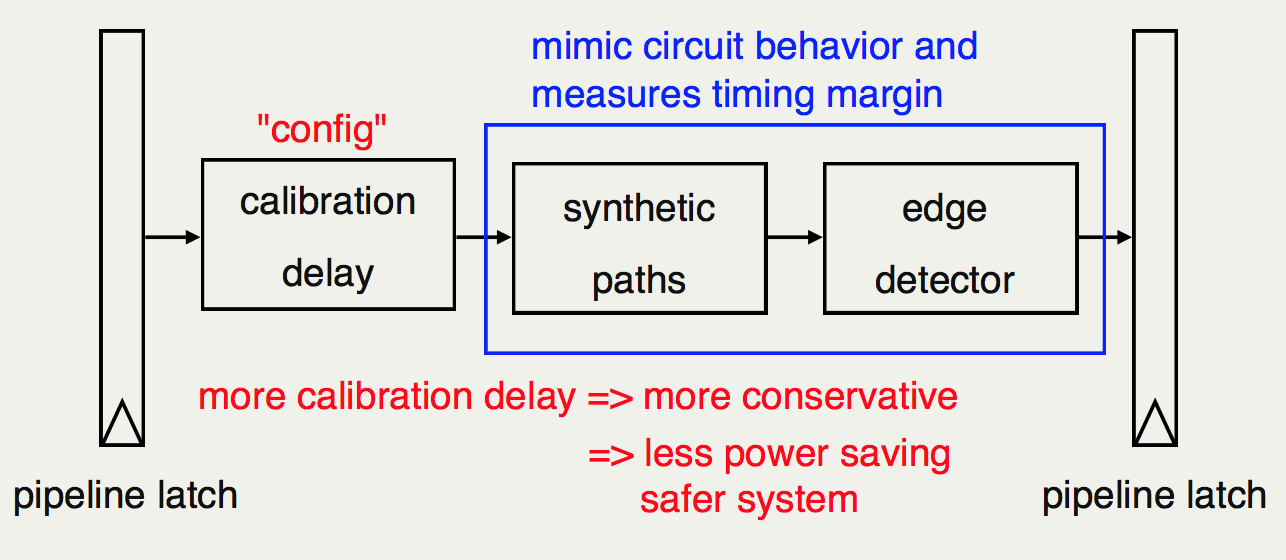
\includegraphics[trim=0 0 0 0, clip, width=0.6\columnwidth]{graphs/cpm-internal.png}
  \caption{Critical Path Monitor's internal structure: it consists of three parts: calibration delay which configures active timing margin's ``safety margin''; synthetic path mimics the real log path; edge detector measures the timing margin left.}
  \label{fig:cpm-internal}
\end{figure}

In a critical path monitor, a signal/edge first starts from a pipeline latch, next it passes through a \textit{calibration delay} stage where some circuit delay is added, then goes through a set of synthetic paths which mimics the processor's real logic circuit, and finally travels through the edge detector which counts how much timing margin is left. The data reported by the edge detector instructs active timing margin's decision logic to determine how to take actions to save power or increase reliability. In this process, adding ``calibration delay'' serves as a stage that adds ``safety margin'' - the more calibration delay added, the less timing margin will be read by the edge detector, and active timing margin will make more conservative decisions. In summary, adding calibration delay in CPM, or adding safety margin in active timing margin processors will reduce the power efficiency gain. This is intuitive because the intent of active timing margin is to reduce redundant margin as much as possible. However, for reliability purpose, some amount of safety margin is still needed.

\begin{figure}[t]
  \centering
  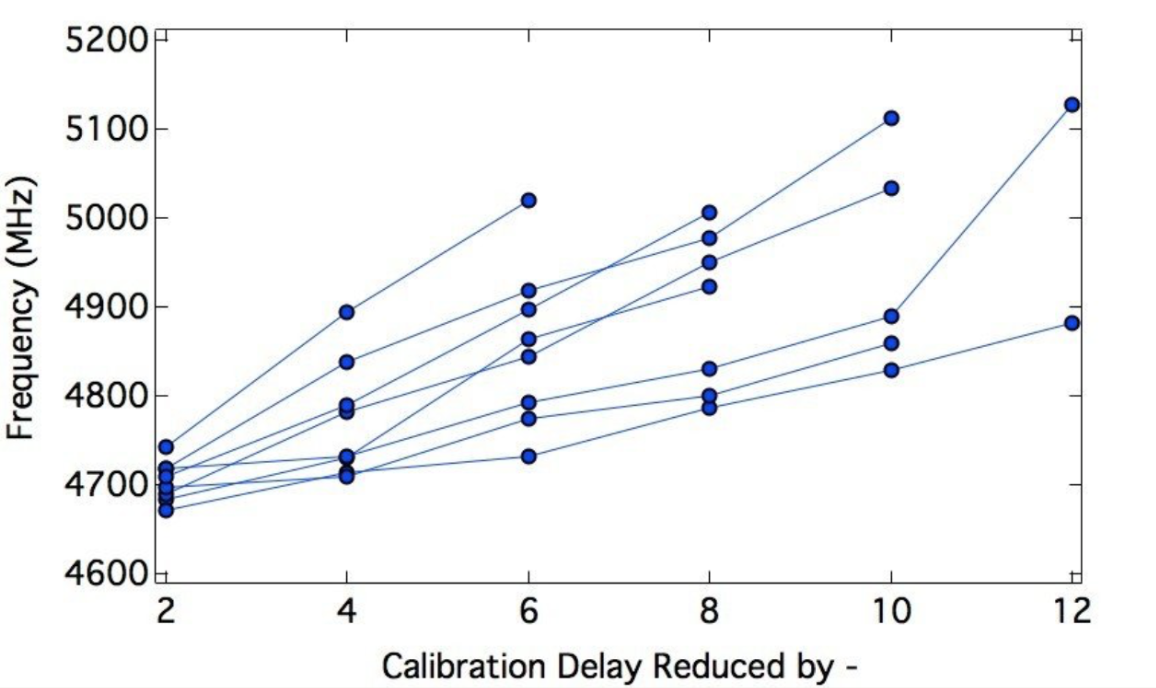
\includegraphics[trim=0 0 0 0, clip, width=0.6\columnwidth]{graphs/cpm-delay-frequency.png}
  \caption{Reducing safety margin can almost double the gain of active timing margin, measured in overclocking benefit.}
  \label{fig:cpm-delay-frequency}
\end{figure}

\Fig{fig:cpm-delay-frequency} illustrates reducing calibration delay in CPM, or reducing safety margin's impact on active timing margin. Here we use POWER7+'s active timing margin for overclocking to boost performance. The static margin's baseline frequency is 4200~MHz. The default active timing margin boost core clock frequency to around 4600~MHz. In~\Fig{fig:cpm-delay-frequency}, we reduce the safety margin by POWER7+'s defined unit of calibration delay, and each line represents the result of one core. We find that reducing safety margin keeps improving active timing margin's performance gain, reaching over 5000~MHz which cannot possibly be set with the conventional static margin.

Another observation we make in~\Fig{fig:cpm-delay-frequency} is that each core has a different characteristics when safety margin is reduced. Some core has a higher overclocking limit and increase frequency faster, compared to others. We highlight the core-to-core variation in~\Fig{fig:cpm-delay-variation}.

\begin{figure}[t]
  \centering
  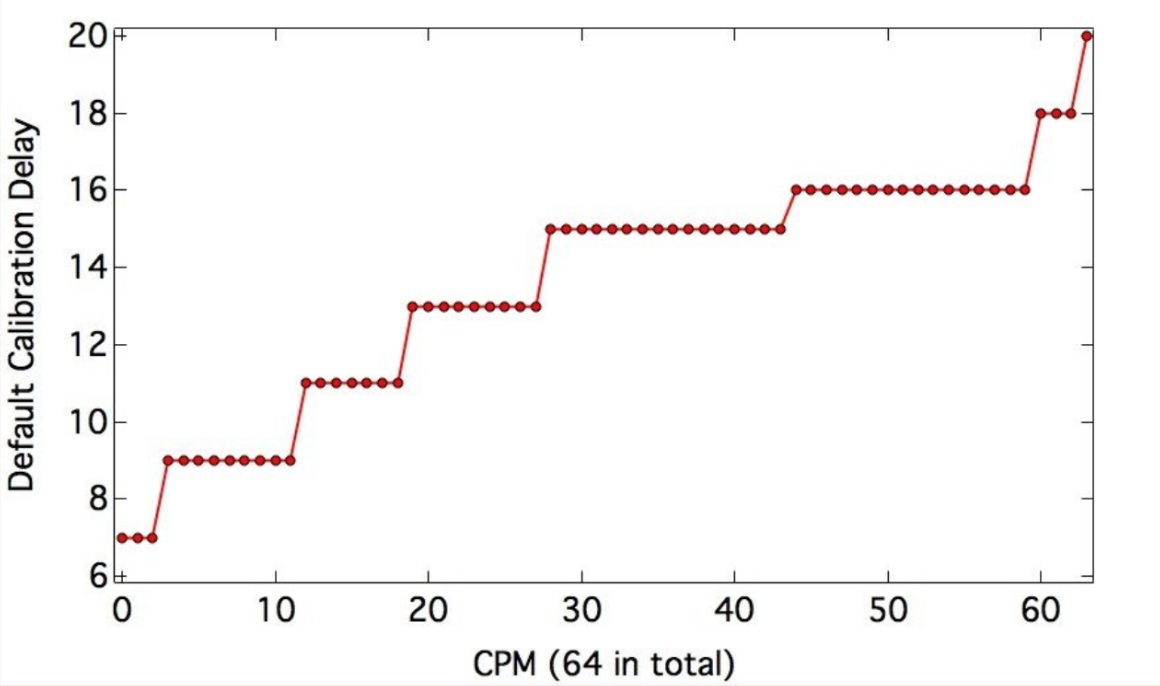
\includegraphics[trim=0 0 0 0, clip, width=0.6\columnwidth]{graphs/cpm-delay-variation.png}
  \caption{Safety margin added to POWER7+'s active timing margin, measured by CPM's defined unit of time delay. Across two processor's 64 CPMs, we observe a wide range of }
  \label{fig:cpm-delay-variation}
\end{figure}

\Fig{fig:cpm-delay-variation} shows the safety margin added to each CPM of the two POWER7+ chips, measured by POWER7+'s self-defined time unit for CPM. The added margin vary by 1X across different CPMs. This is intuitive in that it reflects the process variation within the chip. 

\begin{figure}[t]
  \centering
  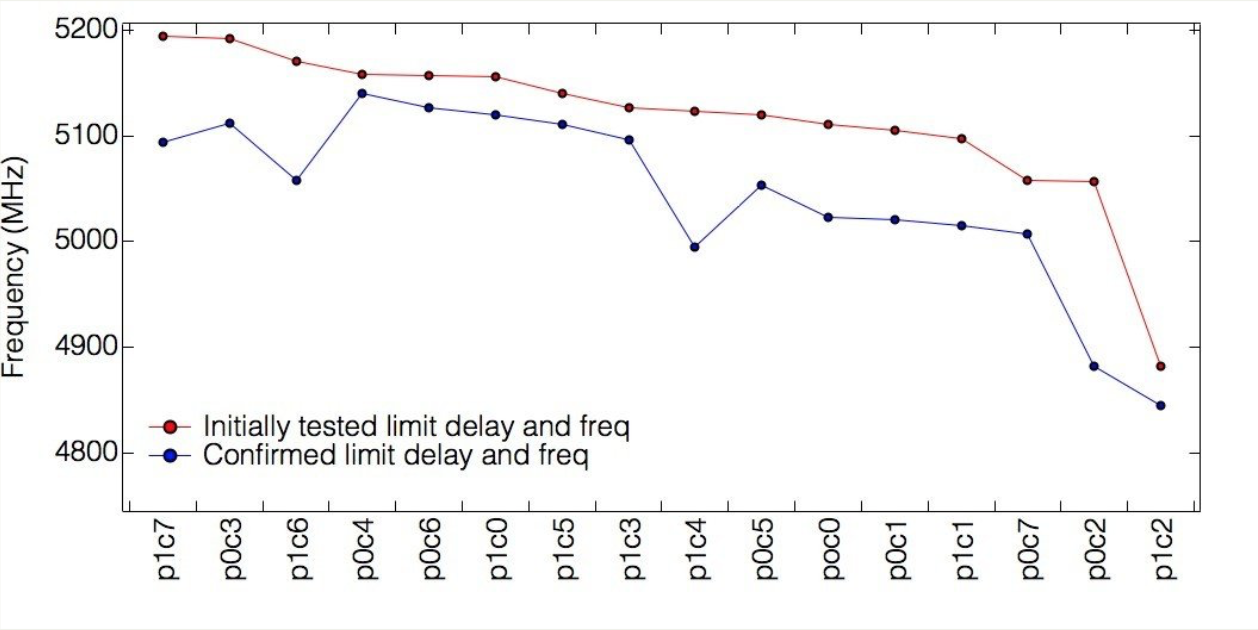
\includegraphics[trim=0 0 0 0, clip, width=0.8\columnwidth]{graphs/cpm-limit-freq.png}
  \caption{The ``limit frequency'' of each core when aggressively reducing the safety margin. The system would crash if safety margin is reduced further, which gives active timing margin's control loop very stringent time to respond. The processor is kept idle in this experiment.}
  \label{fig:cpm-limit-freq}
\end{figure}

We explore the ``limit'' of reducing active timing margin's safety delay when we do not run any workload, i.e., system idle. This gives us an intuition of the limit to operate the processor, and it shows the core-to-core variation. In~\Fig{fig:cpm-limit-freq} we see the limit frequency of all cores are much higher than active timing margin's original overclocking rate of 4600~MHz. However, different cores have diverse limit frequency, which exposes the opportunities from core-to-core variation.

For next step, we can proceed with the following steps:

\begin{itemize}
  \item \textsc{Workload limit frequency analysis} The limit frequency study we conducted so far is constrained to processor idle state. We need to extend this analysis to different single and multi-thread workloads. The purpose is to find the pattern between relationship characteristics and active timing margin's needed safety margin, if there is any. In this process, temperature, voltage, and process variation all comes into play. There will be ``benign'' cores which have higher limit frequency. There will be ``benign'' workloads as well, which does not induce excess timing margin consumption.
    
  \item \textsc{Predicting workload-specific safety margin ~~} After we understand the relationship between workload and active timing margin's safety margin, we can predict the amount of safety margin to be set for each workload. This enables workload specific aggressive active timing margin operation to further improve power efficiency beyond the default active timing margin.
    
  \item \textsc{Devising voltage virus against active timing margin} If we can understand what causes workload to be ``vicious'', we can devise workload that specifically create severe workload to stress active timing margin's control loop. This may lead to a new security threat. We can devise protection mechanism that guards against this threat.
  
\end{itemize}

